% ========================================= TEMPLATE INFO ========================================
%
% Author:       P4ntomime
% Version:      1.0.0
% Last updated: 2024-02-18
% Brief:        A LaTeX template for summaries. See README.md for more information.
% 
% ================================================================================================
\documentclass[8pt, a4paper, twoside]{extarticle}
% Font size:    8pt
% Paper size:   A4
% style:        twoside (needed, so odd and even pages have different margins)
% orientation:  portrait. (use 'landscape' for landscape orientation)


% ========================================= DOCUMENT INFO =========================================
\def\title{Regelungstechnik 2}                                      % title
\def\shorttitle{RegT 2}                                             % short title (displayed as PDF title)
\def\dozent{Prof. Dr. Lukas Ortmann}                                % lecturer
\def\semester{FS 24}                                                % semester
\def\author{Simone Stitz, Laurin Heitzer}                           % author(s)
\def\repo{https://github.com/P4ntomime/regelungstechnik-2}          % repository link
\def\version{1.0.\today}                                            % version
\def\pagelimit{20}                                                  % page limit -> causes pages after limit to be red


% ================================= PACKAGES, SETUP AND COMMANDS ==================================
\input{preamble.tex}


% =========================================== DOCUMENT ============================================
\begin{document}
    \begin{layout}
        \section{Regelkreise aus LTI-Systemen}{105}

\subsection{Steuerung} 
    
    \begin{minipage}[c]{0.48\columnwidth}
        \includegraphics[align=center, width=\columnwidth]{images/steuerung.jpg}
    \end{minipage}
    \hfill
    \begin{minipage}[c]{0.5\columnwidth}
        Eine Steuerung besitzt \textbf{keine Rückkopplung} und ist somit ein \textbf{offener Regelkreis}
        $$ y = \underbrace{K L \cdot r}_{\text{Sensitivität}} + \underbrace{K \cdot z}_{\text{Störung}}$$
    \end{minipage}


\subsection{Regelung}

    \begin{minipage}[c]{0.48\columnwidth}
        \includegraphics[align=center, width=\columnwidth]{images/regelung.jpg}
    \end{minipage}
    \hfill
    \begin{minipage}[c]{0.5\columnwidth}
        Eine Regelung besitzt eine \textbf{Gegenkopplung}
        $$ y = K H \cdot (r - y) + K \cdot z$$
        $$ y = \underbrace{\frac{K H}{1 + K H} \cdot r}_{\text{Sensitivität}} + \underbrace{\frac{K}{1 + K H} \cdot z}_{\text{Störungsunterdrückung}} $$
    \end{minipage}


\subsubsection{Störungsunterdrückung}{106}

    Ein Regler ist vorteilhaft, um Störungen zu unterdrücken, denn für die Verstärkung $H$ der Störung $z$ gilt:
    $$ \lim\limits_{H \to \infty} \frac{K}{1 + K H} \cdot z = 0 $$
    \textrightarrow\ Hat der Regler eine grosse Verstärkung $H$, so wird die Störung $z$ unterdrückt\\
    \textrightarrow\ Bei einer Steuerung wird die Störung $z$ nicht unterdrückt


\subsubsection{Sensitivität (Empfindlichkeit)}{106}

    Für die Sensitivität eines Reglers gilt:
    $$ \lim\limits_{H \to \infty} \frac{K H}{1 + K H} \cdot r = 1 $$
    \textrightarrow\ Hat der Regler eine grosse Verstärkung $H$, so ist $y \approx r$ (Ausgang $\approx$ Sollwert)\\
    \textrightarrow\ Bei einer Steuerung muss $H = \frac{1}{L}$ sein, damit $y \approx r$


\subsubsection{Stabilitätsproblem}{109-110}

    Sobald ein offener Regelkreis (Steuerung) geschlossen wird, muss darauf geachtet werden, dass das System stabil ist.
    

\subsection{Stabilität eines Systems mit Rückkopplung}

    \begin{tabular}{lll}
        (asymp.) stabil     & Verstärkung $|V| < 1$ & System schwingt nicht \\
        grenzstabil         & Verstärkung $V = -1$  & System schwingt mit konstanter Ampl.\\
        instabil            & Verstärkung $|V| > 1$ & System schwingt mit zunehmender Ampl. 
    \end{tabular}


\subsubsection{Berechnung Grenzstabilität}{111}

    Für Grenzstabilität muss für die Verstärkung des Systems gelten: $V = -1$ 


    \example{Grenzstabilität System aus I-Glied und Totzeitglied}

    \begin{center}
        \includegraphics[align=center, width=0.75\columnwidth]{images/gegengekoppeltes_system.png}
    \end{center}

    Es muss gelten: $y(t) = -e(t)$ unter der Annahme, dass $e(t) = A \cdot \cos(\omega t)$

    \vspace*{-0.3cm}        % reduce space before align environment

    \begin{align*}
        x(t) &= K \cdot \int\limits_0^t e(\tau) \diff \tau + x_0 
            = K \cdot \int\limits_0^t A \cdot \cos(\omega \tau) \diff \tau + x_0
            = K \frac{A}{\omega} \sin(\omega \tau) \Big|_0^t + x_0 \\
            &= \frac{K A}{\omega} \sin(\omega t) + \underbrace{x_0}_{0} \\
        y(t) &= x(t - T_t) = \frac{K A}{\omega} \sin(\omega (t - T_t)) = \frac{K A}{\omega} \cos \big( \omega( t- T_t) - \frac{\pi}{2}  \big)
    \end{align*}

 

    $$ \text{Koeffizientenvergleich: } \underbrace{ \cbl{ \frac{K A}{\omega}} \cos \big( \omega t \cor{- \omega T_t - \frac{\pi}{2}}  \big) }_{y(t)}
         = - A \cos(\omega t) = \underbrace{ \cbl{A} \cdot \cos(\omega t \cor{- \pi}) }_{-e(t)} $$
    
    $$ \text{Der Koeffizientenvergleich liefert: } \cbl{\omega = K} \quad \text{und} \quad \cor{\omega = K = \frac{\pi}{2 \cdot T}} $$

    \textrightarrow\ Wenn der Regler die Verstärkung $K$ hat ist das System grenzstabil 
    und das System schwingt für alle Zeit mit der Frequenz $\omega$\\
    \textrightarrow\ Die Verstärkung $K$ muss vermieden werden!

    
        \section{Frequenzgang}{114} 

Wird ein Sinus-Signal $u(t)$ in ein LZI-System gegeben, so ist das Ausgangssignal $y(t)$ wieder sinusförmig.
Dabei ändern sich meist die \textbf{Amplitude} und die \textbf{Phase}.
Die \textbf{Frequenz} hingegen bleibt \textbf{gleich}.\\
Die Amplitude und die Frequenz des Ausgangssignals (bzw. deren Änderung) kann allerdings frequenzabhängig sein!

\begin{minipage}[c]{0.48\columnwidth}
    \includegraphics[width=\columnwidth]{images/lzi_system.png}
\end{minipage}
\hfill
\begin{minipage}[c]{0.48\columnwidth}
    \begin{tabular}{ll}
        $A$             & Amplitude Eingangssignal \\
        $B$             & Amplitude Ausgangssignal \\
        $\frac{B}{A}$   & Verstärkung \\
        $\varphi$       & Phasenverschiebung \\
    \end{tabular}
\end{minipage}

\fbox{\parbox{0.8\columnwidth}{
\begin{tabular}{l c l}
    $ u(t) = A \cdot \cos(\omega t) $ & & $ y(t) = B \cdot \cos(\omega t + \varphi) + \text{Transiente} $
\end{tabular}
}}

\subsubsection*{Transiente}

 Die Transiente beschreibt den Vorgang, bis der eingeschwungene Zustand (\textbf{steady state}) erreicht ist.
 In der Praxis betrachtet man häufig $t = 5 \tau$ als Ende des Einschwingvorgangs \\
 \textrightarrow\ \textbf{Uns interessiert nur der der steady state!}


\subsubsection*{Darstellung des Frequenzgangs}

% Der Frequenzgang stellt die Informationen zu einem System im Frequenzbereich dar. Es handelt sich hierbei um dieselben Informationen
% wie im Zeitbereich. Allerdings sind die Berechnungen im Frequenzbereich wesentlich einfacher als im Zeitbereich \\
Der Frequenzgang kann mittels folgenden Diagrammen dargestellt werden: 

\begin{itemize}
    \item Nyquist-Plot (Ortskurve)
    \item Bode-Plot
    \item Zeiger-Diagramm
\end{itemize}


\subsection[Frequenzgang G(j omega) als komplexe Zahl]{Frequenzgang $G(\jimg \omega)$ als komplexe Zahl}{116}

\vspace{-0.3cm} % reduce space 
$$ \boxed{ G(\jimg \omega) =  \abs{G(\jimg \omega)} \cdot \e^{\jimg \angle G(\jimg \omega)} = \frac{B}{A} \cdot \e^{\jimg  \varphi} } $$


\subsection{Frequenzgang der Grundglieder}

\includegraphics[width=\columnwidth]{images/frequenzgaenge_grundglieder.png} \\
\textrightarrow\ Zusammengesetzte Grundglieder: siehe Skript S. 204-208


\subsection{Darstellung mit Zeigern}

Im Frequenzbereich kann ein Signal \textbf{bei einer bestimmten Frequenz} als Zeigerdiagramm dargestellt werden.
Dabei wird das Signal $\underline{y}(t)$ als Zeiger $\underline{Y}$ zur Zeit $t=0$ dargestellt, welcher anschliessend mit Frequenz $\omega = 2 \pi f$ rotiert.
Das zeitliche Signal $y(t)$ entspricht dem \textbf{Realteil} von $\underline{y}(t)$

\begin{minipage}[c]{0.4\columnwidth}
    \includegraphics[width=\columnwidth]{images/zeigerdiagramm_1.png}
\end{minipage}
\hfill
\begin{minipage}[c]{0.4\columnwidth}
    \includegraphics[width=\columnwidth]{images/zeigerdiagramm_2.png}
\end{minipage}


\subsubsection{Komplexe Amplitude $Y$}

\vspace{-0.5cm} % reduce space before align environment
\begin{align*}
    \underline{y}(t) &= B \cdot [\cos(\omega t + \varphi) + \jimg \sin(\omega t + \varphi)] \\
                &= B \cdot e^{\jimg(\omega t + \varphi)} = \cbl{B \cdot e^{\jimg \varphi}} \cdot e^{\jimg \omega t} \\
                &= \cbl{\underline{Y}} \cdot e^{\jimg \omega t}
\end{align*}

Die in der Gleichung vorkommenden Grössen sind definiert als \\
\begin{tabular}{lll}
    $ | \underline{y}(t) | = B$                 & Maximale Amplitude des Ausgangssignals \\
    $ \mathrm{Re}(\underline{y}(t)) = y(t)$     & Ausgangssignal (zeitlich) \\
    $ \underline{y}(0) = \cbl{\underline{Y}} $  & Anfangszeiger (komplexe Amplitude)
\end{tabular}


\subsubsection{Ableitung / Integral im Frequenzbereich}

\begin{minipage}[c]{0.48\columnwidth}
    $$ \boxed{ \underline{\dot{y}}(t) = \underline{Y} \cdot \jimg \omega \cdot \e^{\jimg \omega t} } $$
\end{minipage}
\hfill
\begin{minipage}[c]{0.48\columnwidth}
    $$\boxed{ \int y(t) \, \diff t = \frac{\underline{Y}}{\jimg \omega} \cdot \e^{\jimg \omega t} } $$
\end{minipage}


\subsection{Bestimmung des Frequenzgangs aus DGL}

\begin{enumerate}
    \item DGL des Systems in Frequenzbereich transformieren
    \item Geeignet umformen: $G(\jimg \omega) = \frac{\underline{Y}}{\underline{U}}$
    \item Falls gewünscht: Amplitude $|G(\jimg \omega)|$ und Phase $\varphi$ bestimmen
\end{enumerate}


\example{$\text{PT}_1$ Glied}

\vspace{-0.3cm} % reduce space
$$ T \dot{y} + y(t) = K u(t) \quad \underrightarrow{\text{Frequenzbereich}} \quad 
T \cdot \jimg \omega \cdot \underline{Y} + \underline{Y} = [\jimg \omega T + 1] \cdot \underline{Y} = K \underline{U} $$
$$ \frac{\underline{Y}}{\underline{U}} = \frac{K}{\jimg \omega T + 1} = G(\jimg \omega) $$
$$ |G(\jimg \omega)| = \frac{|\underline{Y}|}{|\underline{U}|} = \frac{K}{\sqrt{(\omega T)^2 + 1^2}} \qquad \varphi = \frac{K}{1 + (\omega T)^2} - \jimg \frac{K \omega T}{1 + (\omega T)^2 } + \pi $$


\subsubsection{Allgemeiner Fall}


\vspace{-0.5cm} % reduce space before align environment
\begin{align*}
    a_n y(t)^{(n)} + \cdots  + a_1 \dot{y}(t) + a_0 y(t) &= b_m u(t)^{(m)} + \cdots + b_1 \dot{u}(t) + b_0 u(t) \\
    a_n (\jimg \omega)^n \cdot \underline{Y} + \cdots + a_1 \jimg \omega \cdot \underline{Y} + a_0 \underline{Y} 
    &=  b_m (\jimg \omega)^m \cdot \underline{U} + \cdots + b_1 \jimg \omega \cdot \underline{U} + b_0 \underline{U} \\
    \frac{\underline{Y}}{\underline{U}} 
    &= \frac{b_m (\jimg \omega)^m + \cdots + b_1 \jimg \omega + b_0}{a_n (\jimg \omega)^n + \cdots + a_1 \jimg \omega + a_0} = G(\jimg \omega) \\
    |G(\jimg \omega)| = \frac{|\underline{Y}|}{|\underline{U}|}
    &= \frac{| b_m (\jimg \omega)^m + \cdots + b_1 \jimg \omega + b_0 |}{| a_n (\jimg \omega)^n + \cdots + a_1 \jimg \omega + a_0 |} \\
    \varphi = \angle G(\jimg \omega) &= \arctan \left\lgroup \frac{\mathrm{Im} \{G(\jimg \omega)\}}{\mathrm{Re}\{G(\jimg \omega)\}} \right\rgroup (+ \pi)
\end{align*}




\subsection{Serieschaltung von LZI-Systemen}

\begin{center}
    \includegraphics[width=0.7\columnwidth]{images/frequenzgang_serieschaltung.png}
\end{center}
$$ \boxed{ \underline{Y} = \underbrace{G_1(\jimg \omega) \cdot G_2(\jimg \omega)}_{G(\jimg \omega)} \cdot \underline{U} } $$
$$ G_1 \cdot G_2 = |G_1| \cdot \e^{\jimg \angle G_1} \cdot |G_2| \cdot \e^{\jimg \angle G_2} = |G_1| |G_2| \cdot \e^{\jimg (\angle G_1 + \angle G_2)} $$


\subsection{Parallelschaltung von LZI-Systemen}

\begin{center}
    \includegraphics[width=0.5\columnwidth]{images/frequenzgang_parallelschaltung.png}
\end{center}
$$ \boxed{ \underline{Y} = \underline{Y}_1 + \underline{Y}_2 = G_1(\jimg \omega) \cdot \underline{U} + G_2(\jimg \omega) \cdot \underline{U} 
    = \underbrace{(G_1(\jimg \omega) + G_2(\jimg \omega))}_{G(\jimg \omega)} \cdot \underline{U}} $$
$$ G_1 + G_2 = \mathrm{Re}\{ G_1 \} + \mathrm{Re}\{ G_2 \} + \jimg ( \mathrm{Im}\{ G_1 \} + \mathrm{Im}\{ G_2 \}) $$


\subsection{Kreisschaltung (Gegenkopplung) von LZI-Systemen}

\begin{minipage}[c]{0.5\columnwidth}
    \includegraphics[width=\columnwidth]{images/frequenzgang_kreisschaltung.png}
\end{minipage}
\hfill
\begin{minipage}[c]{0.48\columnwidth}
    $$ \boxed{ \underline{Y} = \underbrace{\frac{G_1(\jimg \omega)}{1 + G_1(\jimg \omega) \cdot G_2(\jimg \omega)}}_{G(\jimg \omega)} \cdot \underline{U}} $$
    \textrightarrow\ Anwendung von \textbf{Mason Regel} (SigSys)
\end{minipage}


\subsubsection{Vorgehen Frequenzgang ermitteln}
\begin{enumerate}
    \item Gleichung zum Blockdiagramm aufstellen
    \item Nach $\underline{Y}$ umformen 
\end{enumerate}

\subsection{Frequenzgang -- Übertragungsfunktion (UTF)}

Der Frequenzgang $G(\jimg \omega)$ und die Übertragungsfunktion $G(s)$ mit $s = \sigma + \jimg \omega$ hängen folgendermassen zusammen:
$$ \boxed{G(\jimg \omega) = G(s) \big\vert_{s = \jimg \omega}} $$

\subsubsection{Übersicht Darstellungsformen}

\begin{center}
    \includegraphics[width=0.75\columnwidth]{images/darstellungen_frequenzgang_utf.png}
\end{center}


        \section{Stabilität -- Nyquistkriterium}{126}
\label{offener Regelkreis}

Die Stabilität eines Regelkreises kann mit dem Nyquistkriterium viel einfacher betrachtet werden. 
Dafür wird der \textbf{Frequenzgang} $\bm{G_0(\jimg \omega)}$ \textbf{des offenen Regelkreises} betrachtet.

Ausserdem gibt das Nyquistkriterium an, wie robust ein Regelkreis ist.

\begin{minipage}[c]{0.48\columnwidth}
    \includegraphics[width=\columnwidth]{images/offener_regelkreis.png}
\end{minipage}
\hfill
\begin{minipage}[c]{0.48\columnwidth}
    \begin{center}
        Frequenzgang des offenen Regelkreises
    \end{center}
    $$ \boxed{ G_0(\jimg \omega) = \frac{\underline{Y}}{\underline{E}} } $$
\end{minipage}



\example{Kreisschaltung mit mehreren Blöcken}
\label{Kreisschaltung mehrere Bloecke}

Folgendes System besitzt ein Eingangssignal $\underline{R}$ und vier Ausgangssignale $\underline{Y}$\\
Es sollen der Frequenzgang des offenen Regelkreises $G_0(\jimg \omega)$, sowie ausgewählte UTFs des Systems beschrieben werden.

$$ G_0(\jimg \omega) = G_1(\jimg \omega) \cdot G_2(\jimg \omega) \cdot G_3(\jimg \omega)  $$

\begin{minipage}[c]{0.5\columnwidth}
    \includegraphics[width=\columnwidth]{images/kreisschaltung_mehrere_bloecke.png}
\end{minipage}
\hfill
\begin{minipage}[c]{0.48\columnwidth}
    $$ \frac{\underline{Y}_1}{\underline{R}} = \frac{1}{1 + G_1(\jimg \omega) \cdot G_2(\jimg \omega) \cdot G_3(\jimg \omega)} $$
    % $$ \frac{\underline{Y}_1}{\underline{R}} = \frac{G_1(\jimg \omega)}{1 + G_1(\jimg \omega) \cdot G_2(\jimg \omega) \cdot G_3(\jimg \omega)} $$
    $$ \frac{\underline{Y}_3}{\underline{R}} = \frac{G_1(\jimg \omega) \cdot G_2(\jimg \omega)}{1 + G_1(\jimg \omega) \cdot G_2(\jimg \omega) \cdot G_3(\jimg \omega)} $$
    % $$ \frac{\underline{Y}_4}{\underline{R}} = \frac{G_1(\jimg \omega) \cdot G_2(\jimg \omega) \cdot G_3(\jimg \omega)}{1 + G_1(\jimg \omega) \cdot G_2(\jimg \omega) \cdot G_3(\jimg \omega)} $$
\end{minipage}

\vspace{0.2cm}
\textbf{Hinweis:} Die Stabilität des Systems ist \textbf{unabhängig von der Reihenfolge der Teilsysteme} $G_{i}(\jimg \omega)$,
da die Stabilität durch den Nenner (bzw. die Polstellen) beschrieben wird.


\subsection{Stabilität im Nyquist-Diagramm}

Gedankenexperiment: Ein offener Regelkreis mit $G_0(\jimg \omega)$ (gemäss Abschnitt ~\ref{offener Regelkreis}) um eine 
veränderbare Verstärkung $K$ ergänzt.


\subsubsection{Stabilität}

Wähle $K = K_0$, sodass sich die Ortskurve immer innerhalb des Einheitskreises befindet.
\vspace{0.1cm}
\begin{itemize}
    \item Befindet sich die Ortskurve eines Systems immer \textbf{innerhalb des Einheitskreises}, so ist der offene Regelkreis stabil. \\
        \textrightarrow\ Daraus folgt, dass auch der geschlossene Regelkreis stabil sein muss.
    \item Führungsübertragungsfunktion für $K \ll K_0$:\\
    $G_f(\jimg \omega) = \frac{K \cdot G_0(\jimg \omega)}{1 + K \cdot G_0(\jimg \omega)} \approx K \cdot G_0(\jimg \omega)$ 
\end{itemize}


\subsubsection{Grenzstabilität}

Wähle $K = K_{krit} > K_0$, sodass die Ortskurve den Punkt $-1$ schneidet.
\vspace{0.1cm}
\begin{itemize}
    \item Ortskurve des offenen Regelkreises $G_0(\jimg \omega)$ verläuft \textbf{durch den Punkt $\boldsymbol{-1}$}, 
    \item Die Frequenz $\omega_{\pi}$, für die $G_0(\jimg \omega_{\pi})= -1 = \e^{- \pi}$ heisst \textbf{kritische Frequenz}. Mit dieser 
        kritischen Frequenz schwingt das System.
    \item Die Führungsübertragungsfunktion $G_f(\jimg \omega) = \frac { K \cdot G_0(\jimg \omega)}{1 + K \cdot G_0(\jimg \omega)}$ wird bei 
    der kritischen Frequenz zu $G_f(\jimg \omega_{\pi}) = \frac{-1}{1-1} = - \infty $ \textrightarrow\ Grenzstabilität
\end{itemize}


\subsubsection{Instabilität}

Wähle $K > K_{krit}$
\vspace{0.1cm}
\begin{itemize}
    \item Ortskurve verläuft nicht mehr durch den Punkt $-1$
    \item Das System ist instabil
\end{itemize}


\subsection{Vereinfachtes Nyquistkriterium}{127-128}

Idee: Informationen über den \textbf{offenen Regelkreis} verwenden, um die \textbf{Stabillität des geschlossenen Regelkreises} 
zu beurteilen


\subsubsection{Vereinfachtes Nyquistkriterium}

\fbox{\parbox{0.95\columnwidth}{
\begin{itemize}
    \item Gemäss Abschnitt ~\ref{Kreisschaltung mehrere Bloecke}  wird $G_0 = \prod_i G_i$ gebildet aus den seriegeschalteten
        Teilsystemen des offenen Regelkreises \cbl{(\textrightarrow\ Produkt aller $G_i$ \textbf{im Feedback-Loop})}
    \item $G_0$ muss dabei einem \textbf{Prozess mit Ausgleich \cbl{(stabilen Prozess)}} entsprechen; zusätzlich 
    \textbf{dürfen} noch einer oder zwei Integratoren seriegeschaltet sein\\
        Mit Polen formuliert: Bei $G_0$ sind maximal zwei Pole bei Null erlaubt; alle weiteren Pole müssen in der linken Halbebene liegen
    \item Damit der geschlossene Regelkreis stabil ist, muss der kritische Punkt $-1$ \textbf{links} der Nyquistkurve von $G_0$ liegen,
        wenn diese in Richtung zunehmender Frequenz durchlaufen wird ($\omega = 0 \ldots \infty$) 
        \cbl{\textrightarrow\ 'links der Kurve': Man befindet sich \textbf{auf der Kurve} und 'schaut' nach links und muss
        den Punkt $-1$ 'sehen'}
\end{itemize}
}}


\example{Ortskurven stabiler Systeme}{128}

\textbf{Achtung:} Damit die Stabilität der gezeigten Systeme beurteilt werden kann, muss sichergestellt werden, dass auch die ersten
beiden Punkte des vereinfachten Nyquistkriteriums eingehalten werden!

\includegraphics[width=\columnwidth]{images/nyquist_stabile_kurven.png}


\subsection{Stabilitätsreserven}

Wir möchten nicht nur Stabilität, sondern auch eine gewisse Stabilitätsreserve, um z.B. auch bei einem ungenau
modellierten Prozess oder einer sich ändernden Regelstrecke noch einen stabilen Regelkreis zu gewährleisten. 
\vspace{0.2cm}
\begin{outline}
    \1 \textbf{Auch ein stabiler Regelkreis kann sehr lange (ein)schwingen}
    \1 Stabilität / Grenzstabilität / Instabilität sind defnierte Bereiche
        \2 Es gibt nicht 'ein wenig stabil', 'ziemlich stabil', 'stabiler als...', 'instabiler als'
    \1 Allenfalls: Ein Regelkreis ist stabiler als ein anderer. Gemeint ist:
        \2 Ein Regelkreis ist besser gedämpft / schneller (eingeschwungen)
        \2 Ein Regelkreis ist robust -- er ist trotz gewissen Widerigkeiten im Regelkreis
        \2 \textbf{Ein Regelkreis bleibt stabil, auch wenn die Regelstrecke leicht ändert}
\end{outline}


\subsection{Stabilitätsreserven im Nyquistdiagramm}{129}


\begin{minipage}[c]{0.48\columnwidth}
    \includegraphics[width=\columnwidth]{images/stabilitaetsreserven_1.png}
\end{minipage}
\hfill
\begin{minipage}[c]{0.5\columnwidth}

    $$ \boxed{\Phi_{RES} = \arctan \left( \frac{\Re{G_{0}(\jimg \omega_{D})}}{\Im{G_{0}(\jimg \omega_{D})}} \right) } $$
    $$ \boxed{\frac{1}{K_{RES}} = \big| G_{0}(\jimg \omega_{\pi}) \big| } $$


     Ein System ist \textbf{stabil}, wenn eine der folgenden Bedingungen erfüllt ist:
     \vspace{0.2cm}

     \begin{itemize}
        \setlength\itemsep{4pt}
        \item $\omega_{\pi} > \omega_{D}$
        \item $G_{0}(\jimg \omega_{D}) = \e^{- \jimg \varphi}$ \quad mit $0 < \varphi < \pi$
        \item $0 > G_{0}(\jimg \omega_{\pi}) > -1 $
     \end{itemize}
\end{minipage}

\vspace{0.2cm}

\begin{itemize}
    \item Durchtrittsfrequenz $\omega_{D}$ \\
        Frequenz, bei der die Kurve den Einheitskreis durchquert: $| G_{0}(\jimg \omega_{D})| = 1 $ \\
        \textrightarrow\ Phasenreserve $\Phi_{RES}$
    
    \item Phasenschnittfrequenz $\omega_{\pi}$ \\
        Frequenz, bei der die Kurve die reelle Achse durchquert: $\Im{G_{0}(\jimg \omega_{\pi})} = 0$\\
        \textrightarrow\ Verstärkungsreserve $K_{RES}$
\end{itemize}


\subsubsection{Verstärkungsreserve $K_{RES}$}

Die Verstärkungsreserve $K_{RES}$ liefert direkt den Toleranzwert für den Fall, dass die \textbf{Modellunsicherheit} des 
offenen Regelkreises bei der \textbf{Verstärkung} liegt. \\
Der Abstand zur Ursprung bei der Phasenschnittfrequenz $\omega_{\pi}$ entspricht $\frac{1}{K_{RES}}$ \\
\textrightarrow\ Wenn anstatt dem Nominalfrequenzgang $G_0(\jimg \omega)$ tatsächlich $K_{RES} \cdot G_0(\jimg \omega)$ vorliegt, wird der
Regelkreis \textbf{grenzstabil}!


\subsubsection{Phasenreserve $\Phi_{RES}$}

Die Phasenreserve $\Phi_{RES}$ liefert einen Toleranzwert für den Fall, dass die \\
\textbf{Modellunsicherheit} des offenen Regelkreises bei der \textbf{Totzeit} liegt.

\textrightarrow\ Wenn anstatt dem Nominalfrequenzgang $G_0(\jimg \omega)$ tatsächlich $G_0(\jimg \omega) \cdot \e^{- \jimg \omega T_t}$ vorliegt, 
wird der Regelkreis \textbf{grenzstabil}!
\bigskip

Der Zusammenhang zwischen Phasendrehung und Totzeit ist
$$ \boxed{ T_t = \frac{\Phi_{RES}}{\omega_D}  \quad \text{ wobei } [\Phi_{RES}] = \rad } $$


\example{Einfluss von Stabilitätsreserven auf Nyquistdiagramm}

\includegraphics[width=\columnwidth]{images/nyquist_stabilitaetsreserven.png}

\begin{tabular}{ll}
    Mitte:  & Verstärkungsreserve streckt Kurve vom Ursprung aus \\
    Rechts: & Phasenreserve dreht jeden Punkt der Kurve um verschiedene Winkel $\omega \cdot T_t$ \\
            & um den Ursprung  
\end{tabular}


\subsubsection{Faustregeln für Reserven}{131}

\textbf{Hinweis:} Es besteht eine Kopplung zwischen den beiden Effekten!

\begin{itemize}
    \item Phasenreserve von $\Phi_{RES} = 40 \degree \ldots 70 \degree$
    \item Verstärkungsreserve von $K_{RES} > 4 \, (\approx 12 \, \deci \bel)$
\end{itemize}


\subsection{Nyquistdiagramme mit MatLab}

\lstinputlisting{snippets/nyquist.m}

\subsection{Vorgehen: Nyquistdiagramme zeichnen}

\begin{itemize}
    \item Werte für $G(\omega = 0)$ und $G(\omega = \infty)$ berechnen
    \item Anzahl $\jimg$ im Zähler \textbf{plus} Anzahl $\jimg$ im Nenner entspricht Anzahl Quadranten, welche zwischen $\omega = 0$ und 
        $\omega = \infty$ durchlaufen werden
    \item Pollstellen: $|G(\jimg \omega)|$ \textdownarrow\ ; $\angle G(\jimg \omega)$ \textdownarrow\ \textrightarrow\ Bewegung im Uhrzeigersinn
        \textrightarrow\ Bei den Nullstellen ist $\angle G(\jimg \omega) = \pm 45 \, \degree$
    \item Nullstellen: $|G(\jimg \omega)|$ \textuparrow\ ; $\angle G(\jimg \omega)$ \textuparrow\ ; \textrightarrow\ Bewegung im Gegenuhrzeigersinn
    \item Frequenzen der Pol- bzw. Nullstellen berechnen
\end{itemize}
        \section{Dezibel $\deci \bel$}


\subsection{Umrechnung Verstärkungsfaktor -- Dezibel $\deci \bel$}

$$ \boxed{ |K|_{\deci \bel} = 20 \, \deci \bel \cdot \log_{10} |K| \quad \Leftrightarrow \quad 
            |K| = 10 ^{\big( \frac{|K|_{\deci \bel}}{20 \, \deci \bel}\big)}  } $$

Hinweis: Die Betragsstrichte sind Notation! Es können sehr wohl negative Werte entstehen!

\subsubsection{Rechenregeln}

\begin{itemize}
    \item Multiplikation \textrightarrow\ Addition
    \item Division \textrightarrow\ Subtraktion
    \item Kehrwert \textrightarrow\ Negatives Vorzeichen
\end{itemize}


\subsection{$\deci \bel$--Umrechnungstabelle}

% copy paste from SigSys -> to be updated
\begin{ctabular}{l l}
    \toprule
    \textbf{Dezibel}        & \textbf{Faktor} \\
    \midrule
    $20 = 10 + 10$          & $100 = 10 \cdot 10$ \\ 
    $12$                    & $16 = 2 \cdot 2 \cdot 2 \cdot 2$ \\
    $\cor{10}$              & $\cor{10}$ \\
    $9 = 3 + 3 + 3$         & $8 = 2 \cdot 2 \cdot 2$ \\
    $8 = 5 - 3$             & $6.4 = 3.2 \cdot 2$ \\
    $7 = 10 -3$             & $5 = \frac{10}{2}$ \\
    $6 = 3 + 3$             & $4 = 2 \cdot 2$ \\
    $5 = 15 - 10$           & $3.2 = \frac{32}{10\mathstrut} \approx \sqrt{10}$ \\
    $4 = 10 - 6 = 10 - 3-3$ & $2.5 = \frac{10\mathstrut}{2 \cdot 2}$ \\
    $\cor{3}$               & $\cor{2}$ \\
    $2= 12-10= 5-3$         & $1.6 = \frac{16}{10}$ \\
    $1 = 10 - 3 - 3 - 3$    & $1.25 = \frac{10}{2\cdot 2 \cdot 2} = \frac{5}{4}$ \\
    $\cor{0}$               & $\cor{1}$ \\
    $-1$                    & $0.8 = \frac{4}{5}$ \\
    \bottomrule
\end{ctabular}

        \section{Bode-Diagramm}

Das Bode-Diagramm ist eine weitere Variante, den Frequenzgang $G(\jimg \omega)$ grafisch darzustellen.
Die Darstellung beinhaltet zwei Graphen.

\begin{itemize}
    \item Amplitudengang $|G(\jimg \omega)|$ in Dezibel $\deci \bel$
    \item Phasengang $\angle G(\jimg \omega)$ in Grad $\degree$
    \item Die Frequenzachse ist \textbf{logarithmisch} mit $\log_{10}(\omega)$
    \item \textbf{Ein Bodediagramm kann in ein Nyquistdiagramm umgezeichnet werden, aber nicht umgekehrt!}
\end{itemize}


% Bei zu wenig Platz weglassen
\subsubsection{Logarithmische Frequenzachse}{134}

\begin{outline}
    \1 Serieschaltung von Systemen
        $$ G(\jimg \omega) = G_1(\jimg \omega) \cdot G_2(\jimg \omega) $$

        \2 Amplitudengang
            $$ |G(\jimg \omega)| = |G_1(\jimg \omega)| \cdot |G_2(\jimg \omega)| $$
            $$ |G(\jimg \omega)|_{\deci \bel} = |G_1(\jimg \omega)|_{\deci \bel} + |G_2(\jimg \omega)|_{\deci \bel} $$
            \textrightarrow\ Grafisch multiplizieren wäre schwierig, grafisch addieren geht gut

        \2 Phasengang
            $$ \angle G(\jimg \omega) = \angle G_1(\jimg \omega) +  \angle G_2(\jimg \omega) $$
            \textrightarrow\ Die Phase muss nicht logarithmisch sein, wir haben schon eine Addition 
\end{outline}


\subsection{Vorgehen: Bode-Diagramm zeichnen}
\label{Bodediagramm zeichnen}

Das Diagramm wird approximativ mit \textbf{Geraden} gezeichnet!

\begin{outline}
    \1 Frequenzgang in folgende Form bringen:
        $$ G(\jimg \omega) = K_0 \cdot (\jimg \omega)^v \cdot \frac{(1 + T_{n0} \cdot \jimg \omega)\cdot (1 + T_{n1} \cdot \jimg \omega) \cdot \ldots}
        {(1 + T_{p0} \cdot \jimg \omega)\cdot (1 + T_{p1} \cdot \jimg \omega) \cdot \ldots} \cdot e^{- \jimg \omega T_t} $$
        \2 Für $\omega = 0$ sind alle $(1 + T \cdot \jimg \omega) = 1 = 0 \, \deci \bel$
        \2 Für $\omega = \frac{1}{T}$ sind alle  $(1 + T \cdot \jimg \omega) = 1 + \jimg = \sqrt{2} \cdot e^{\jimg \frac{\pi}{4}} 
            = 3 \, \deci \bel \angle 45 \, \degree$
    \1 Frequenzen der Nullstellen berechnen: $\omega = \frac{1}{T_n}$
    \1 Frequenzen der Polstellen berechnen: $\omega = \frac{1}{T_p}$


    \1 Jede \textbf{Nullstelle} bewirkt
        \2 einen Knick um $+ 20 \, \deci \bel$ / Dekade \textbf{nach oben} im Amplitudengang
        \2 einen Phasenhub von $+ 90 \, \degree$ über 2 Dekaden \textrightarrow\ $+ 45 \, \degree$ beim Knick
    \1 Jede \textbf{Polstelle} bewirkt
        \2 einen Knick um $- 20 \, \deci \bel$ / Dekade \textbf{nach unten} im Amplitudengang
        \2 einen Phasenverlust von $- 90 \, \degree$ über 2 Dekaden \textrightarrow\ $- 45 \, \degree$ beim Knick
    \1 Einzelne Faktoren einzeichnen \textrightarrow\ Wenn Faktor quadriert ist, zwei mal einzeichnen!
    \1 Grafische Addition der Faktoren für gesamten Frequenzgang
\end{outline}


\example{Bode-Diagramm zeichnen}
\vspace{-0.2cm}
$$ G(\jimg \omega) = \frac{\jimg \omega + 10}{(\jimg \omega + 0.1)} \quad  \underrightarrow{\text{ Standardform }} \quad 
  G(\jimg \omega) = \cgn{100} \cdot \frac{(\cvt{1 + 0.1 \, \jimg \omega})}{(\cbl{ 1 + 10 \, \jimg \omega})} $$

  \begin{itemize}
    \item $ \cgn{\abs{K_0}_{\deci \bel} = \abs{100}_{\deci \bel} = 40 \, \deci \bel}$ \textrightarrow\ $\angle G(100) = 0 \, \degree$
    \item Nullstelle: \cvt{$\abs{1 + 0.1 \, \jimg \omega}_{\deci \bel}$} \textrightarrow\ Knick bei $\omega = \frac{1}{0.1 \, \second} = 10 \frac{\rad}{\second}$
    \item Polstelle: \cbl{$\abs{1 + 10 \, \jimg \omega}_{\deci \bel}$} \textrightarrow\ Knick bei $\omega = \frac{1}{10 \, \second} = 0.1 \frac{\rad}{\second}$
    \item \cor{Endresultat}: Grafische Addition der Teilresultate
  \end{itemize}

\begin{center}
    % Gain
    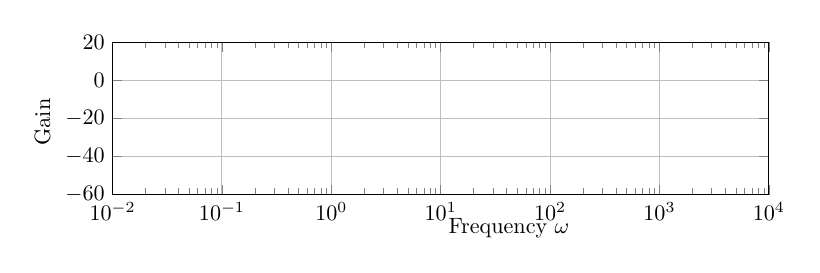
\begin{tikzpicture}
        [
            scale = 0.8,
            >=latex
        ]
        \begin{axis}
            [
                width=12cm,
                height=4cm,
                xmode=log,
                xmin=0.01, xmax=10000, ymin=-60, ymax=20,
                x label style={anchor=west},
                xlabel=Frequency $\omega$,
                y label style={anchor=south},
                ylabel=Gain $\deci \bel$,
                grid
            ]
            
            % coordinates
            
            % draw connections

            
           
        \end{axis}
        
    \end{tikzpicture}

    \vspace{0.3cm}


    % Phase
    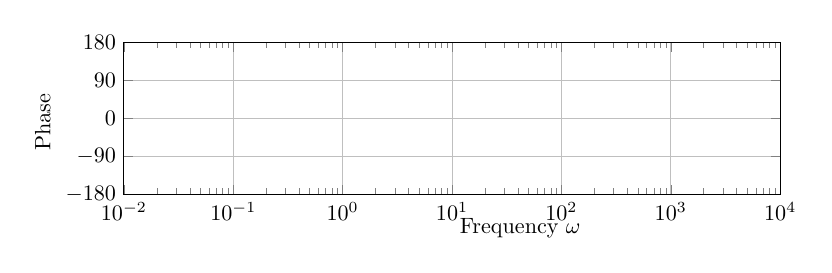
\begin{tikzpicture}
        [
            scale = 0.8,
            >=latex
        ]
        \begin{axis}
            [
                width=12cm,
                height=4cm,
                xmode=log,
                xmin=0.01, xmax=10000, ymin=-180, ymax=180,
                x label style={anchor=west},
                xlabel=Frequency $\omega$,
                y label style={anchor=south},
                ylabel=Phase $\degree$,
                ytick={-180, -90, 0, 90, 180},
                % yticklabels={-180, -90, 0, 90, 180},
                grid
            ]
            
            % coordinates
            
            % draw connections

            
            
        \end{axis}
            
    \end{tikzpicture}
\end{center}


\subsubsection{Inverse Frequenzgänge}{137}

Um das Bodediagramm des inversen Frequenzgangs $\frac{1}{G(\jimg \omega)}$ zu erhalten, muss bei Betrag \textbf{und} Phase
das \textbf{Vorzeichen gedreht} werden.
\vspace{0.2cm}
 
\includegraphics[width=\columnwidth]{images/inverse_frequenzgaenge.png}


\subsubsection{Lead-Lag-Glied}
\label{Lead-Lag-Glied}

$$ \boxed{ \text{Lead-Lag-Glied: } \quad G(s) = K \cdot \frac{s T_1 + 1}{s T_2 + 1} } $$

\begin{minipage}[c]{0.48\columnwidth}
    \begin{center}
        \myul{Lead-Glied ($T_1 > T_2$)}
    \end{center}
    \includegraphics[width=\columnwidth]{images/bode_lead-glied.png}
\end{minipage}
\hfill
\begin{minipage}[c]{0.48\columnwidth}
    \begin{center}
        \myul{Lag-Glied ($T_2 > T_1$)}
    \end{center}
    \includegraphics[width=\columnwidth]{images/bode_lag_glied.png}
\end{minipage}

$$ \boxed{ \text{Maximale Phasenänderung bei:} \quad \omega = \frac{1}{\sqrt{T_1 \cdot T_2}} } $$
\textrightarrow\ Bei der Regler-Auslegung werden vor allem Lead-Glieder verwendet, um \textbf{Phase anheben} zu können


\subsection{Modellbildung (UTF) mittels Frequenzmessung}{139}

Um aus einem gegebenen Bodediagramm die Übertragungsfuntion $G(\jimg \omega)$ zu ermitteln, werden die Zeichenregeln aus Abschnitt
~\ref{Bodediagramm zeichnen} \textbf{rückwärts angewendet}. Dazu werden die Punkte einer gegebenen Messung mittels Geraden approximiert.
Mittels dieser Approximationen können die einzelen Komponenten (Faktoren) der gesuchten UTF ermittelt werden.


\example{Übertragungsfuntion $G(s)$ aus Bodediagramm ermitteln}

\begin{minipage}[c]{0.5\columnwidth}
    \includegraphics[width=\columnwidth]{images/bode_zu_modell.png}
\end{minipage}
\hfill
\begin{minipage}[c]{0.48\columnwidth}
    Aus den Steigungen der Geraden ist ersichtlich, dass folgende Komponenten in $G(s)$ enthalten sein müssen: \\
    \cor{Verstärkung $K$}, \cgn{$\text{PT}_1$-Glied}, \textcolor{cyan}{$\text{PT}_2$-Glied}
    $$ G(s) = \cor{K} \cdot \cgn{\frac{1}{(s T_1 + 1)}} \cdot \textcolor{cyan}{\frac{1}{(T_2^2 s^2 + 2 \zeta T_2 s + 1)}} $$
    Werte der Parameter aus Bodediagramm bestimmen:
    \begin{itemize}
        \item \cor{$|K|_{\deci \bel} = 40$ \textrightarrow\ $K = 100$}
        \item \cgn{$\omega_1 = \frac{1}{T_1} = 0.5$ \textrightarrow\ $T_1 = \frac{1}{0.5} = 2$}
        \item \textcolor{cyan}{$\omega_2 = \frac{1}{T_2} = 10$ \textrightarrow\ $T_1 = \frac{1}{10} = 0.1$}
        \item \textcolor{cyan}{$\zeta = 0.1$} \textrightarrow\ gegeben 
    \end{itemize}
\end{minipage}



\subsection{Stabilität im Bodediagramm}{140}
Analog zum Punkt $-1$ im Nyquistdiagramm kann die Stabilität auch im Bodediagramm beurteilt werden. Auch bei dieser Betrachtung 
sind die folgenden Frequenzen relevant.

\begin{itemize}
    \item Durchtrittsfrequenz $\omega_{D}$ \textrightarrow\ Phasenreserve $\Phi_{\rm RES}$ \\
        Frequenz, bei der die Verstärkung 1 ist: $| G_{0}(\jimg \omega_{D})| = 1 \, (= 0 \, \deci \bel)$
    \item Phasenschnittfrequenz $\omega_{\pi}$ \textrightarrow\ Verstärkungsreserve $\Phi_{\rm RES}$ \\
        Frequenz, bei der die Phase $-180 \, \degree$ beträgt: $\angle {G_{0}(\jimg \omega_{\pi})} = - \pi \, \rad \, (= -180 \, \degree)$
\end{itemize}


\subsubsection[Parameter K_{\rm RES} und  \Phi_{\rm RES} aus Bodediagramm lesen]{Parameter $K_{\rm RES}$ und  $\Phi_{\rm RES}$ aus Bodediagramm lesen}

\begin{minipage}[c]{0.55\columnwidth}
    \includegraphics[width=\columnwidth]{images/bodeplot_stabilitaetsreserven.png}
\end{minipage}
\hfill
\begin{minipage}[c]{0.42\columnwidth}
    \raggedright%
    \begin{itemize}
        \item \cgn{Durchtrittsfrequenz $\omega_{D}$} 
            $$ K_{\rm RES} = 0 \, \deci \bel - K_{\text{@} 180 \degree } $$ 

        \item \cor{Phasenschnittfrequenz $\omega_{\pi}$} 
            $$ \Phi_{\rm RES} = \Phi_{\text{@}0 \deci \bel }  + 180 \, \degree $$ 
    \end{itemize}
    \crd{\textbf{Achtung:} Das Vorzeichen von $\Phi_{\rm RES}$ bzw. $\Phi_{\rm RES}$ ist essentiell für die Stabilitäts-Beurteilung und
    darf auf keine Fall vernachlässigt werden!}
\end{minipage}


\subsubsection{Beurteilung der Stabilität des Systems}

Wenn das System die \textbf{Anforderungen des Nyquist-Kriteriums erfüllt}, verhält sich die Stabilität des Systems folgendermassen:

\begin{itemize}
    \item \textbf{Grenzstabilität}: Amplitudengang bei $0 \, \deci \bel$ \textbf{und} Phasengang bei $-180 \, \degree$
    \item \textbf{Instabilität}:  $K_{\rm RES} < 0$ \textbf{und} $\Phi_{\rm RES} < 0$ (ergibt sich automatisch, wenn einer der 
        beiden Parameter $< 0$ ist)
    \item \textbf{Stabilität}: $K_{\rm RES} > 0$ \textbf{und} $\Phi_{\rm RES} > 0$ 
    \item \textbf{Stabilität}: $\omega_{\pi} > \omega_D$  % gemäss Skript
\end{itemize}


\subsection{Bodediagramme mit Matlab}

\lstinputlisting{snippets/bode.m}


\subsection{Alternative Stabilitätskriterien -- Vorzeichenregel}{142}

Die Stabilität kann alternativ 'direkt' au sden Parametern der \textbf{Differentialgleichung} (des
Frequenzgangs) des \textbf{geschlossenen Regelkreises} bestimmt werden.\\
Aus der DGL der Form
$$ \sum\limits_{k=0}^n a_k \cdot y^{(k)}(t) = \sum\limits_{k=0}^m b_k \cdot u^{(k)}(t) $$
kann das \textbf{charakteristische Polynom} ermittelt werden. Daraus kann dann mittels 
folgender \textbf{Vorzeichenregel} eine Aussage über die Stabilität des \textbf{geschlossenen Regelkreises} 
gemacht werden.

\fbox{\parbox{0.95\columnwidth}{
Eine \textbf{notwendige} Stabilitätsbedingung für das \cbl{charakteristische Polynom}
\begin{align*}
    % \frac{Y}{U}                             &= \frac{\text{Zähler}}{\cbl{a_n \lambda^n + a_{n-1} \lambda_{n-1} + \ldots + a_2 \lambda^2  + a_1 \lambda + a_0 } } \\
    \frac{Y(s)}{U(s)}                       &= \frac{\text{Zähler}}{\cbl{a_n s^n + a_{n-1} s_{n-1} + \ldots + a_2 s^2  + a_1 s + a_0 } } \\
    \frac{Y(\jimg \omega)}{(\jimg \omega)}  &= \frac{\text{Zähler}}{\cbl{a_n (\jimg \omega)^n + a_{n-1} (\jimg \omega)_{n-1} + \ldots + a_2 (\jimg \omega)^2  + a_1 (\jimg \omega) + a_0 } }
\end{align*}
besteht darin, das alle Koeffizienten existieren $a_0 \ldots a_n$ (also $\neq 0$ sind) \textbf{und dasselbe Vorzeichen} haben. \\
Bei System erster und zweiter Ordnung ist die Vorzeichenregel auch \textbf{hinreichend} für die Stabilität.
}}


\example{Stabil, instabil oder 'keine Ahnung'}

\begin{minipage}{0.3\columnwidth}
    \begin{center}
        \textbf{stabil}
    \end{center}
    $$ \frac{1}{\cbl{s^2 + 5s + 7}} $$
\end{minipage}
\hfill
\begin{minipage}{0.3\columnwidth}
    \begin{center}
        \textbf{instabil}
    \end{center}
    $$ \frac{1}{\cbl{s^2 -7s + 3}} $$
\end{minipage}
\hfill
\begin{minipage}{0.3\columnwidth}
    \begin{center}
        \textbf{keine Ahnung}
    \end{center}
    $$ \frac{1}{\cbl{s^3 + 2 s^2 + s + 4}} $$
\end{minipage}


\example{Stabilität aus geschlossenem Regelkreises bestimmen}

\begin{minipage}[c]{0.56\columnwidth}
    \includegraphics[width=\columnwidth]{images/beispiel_regelkreis_vorzeichenkriterium.png}
\end{minipage}
\hfill
\begin{minipage}[c]{0.42\columnwidth}
    \begin{center}
        UTF geschlossener Regelkreis: 
    \end{center}
    $$ \boxed{ T(s) = \frac{Y(s)}{R(s)} = \frac{G_R(s) \cdot G_S(s)}{1 + G_R(s) \cdot G_S(s)} } $$
\end{minipage}

\vspace{0.2cm}
$G_R(s)$ und $G_S(s)$ seien gegeben als: $G_R(s) = K_R, \quad  G_S(s) =\frac{K}{s(sT + 1)} = \frac{K}{T s^2 + s} $
$$ \Rightarrow  T(s) = \frac{G_R(s) \cdot G_S(s)}{1 + G_R(s) \cdot G_S(s)} 
= \frac{\frac{K_R \cdot K}{T s^2 + s}}{1 + \frac{K_R \cdot K}{T s^2 + s}} 
= \frac{K_R \cdot K}{\cbl{T s^2 + s + K_R \cdot K}} \text{\textrightarrow\ stabil für } K_R, K, T > 0 $$


        \section{PID-Regler}

\begin{outline}
    \1 \textbf{P}: Proportional $K_P \cdot e(t)$
        \2 Gegenwart: Gewichtung des \textbf{aktuellen} Fehlers $e(t)$
            \3 Stellgrösse $u(t)$ ist abhängig vom aktuell vorhandenen Fehler $e(t)$
            \3 Wie gross Fehler in Vergangenheit war oder in welche Richtung er sich entwickelt, ist irrelevant
    \1 \textbf{I}: Integral $K_I \int e(t)$
        \2 Vergangenheit: Gewichtung der \textbf{Summe vergangener} Fehler $e(t)$
            \3  Stellgrösse $u(t)$ ist abhängig davon, wie lange ein Fehler schon existiert
            \3 Wie gross der aktuelle Fehler ist und wie start er sich gerade ändert, ist irrelevant
    \1 \textbf{D}: Differential $K_D \cdot \dot{e}(t)$
        \2 Zukunft, Trend: Gewichtung der \textbf{Änderung} des Fehlers $e(t)$
            \3 Stellgrösse ist abhängig davon, wie stark der Fehler gerade zu-/abnimmt
            \3 Wie gross der aktuelle Fehler ist und wie lange er schon existiert, ist irrelevant
\end{outline}


\subsection{Strukturen und Frequenzgänge von PID-Reglern}
\label{Strukturen PID-Regler}

Alle drei Strukturen sind \textbf{äquivalent}. Es handelt sich nur um unterschiedliche Darstellungsformen.


\subsubsection{Varirante 1: Parallelform}
\label{PID-Regler Parallelform}

\begin{minipage}[c]{0.4\columnwidth}
    \includegraphics[width=\columnwidth]{images/pid_regler_aufbau.png}
\end{minipage}
\hfill
\begin{minipage}[c]{0.48\columnwidth}
    $$ \boxed{ G_{\rm PID}(\jimg \omega) = K_P + \frac{K_I}{\jimg \omega} + K_D \frac{\jimg \omega}{1 + \jimg \omega T_C} } $$
\end{minipage}


\subsubsection{Variante 2: Standardform (P-Anteil vorangestellt)}
\label{PID-Regler Standardform}

\begin{minipage}[c]{0.4\columnwidth}
    \includegraphics[width=\columnwidth]{images/pid_regler_aufbau_standardform.png}
\end{minipage}
\hfill
\begin{minipage}[c]{0.55\columnwidth}
    $$ \boxed{ G_{\rm PID}(\jimg \omega) = K_R \cdot \left\lgroup 1 + \frac{1}{\jimg \omega T_N} +\frac{\jimg \omega T_V}{1 + \jimg \omega T_C} \right\rgroup } $$
\end{minipage}


\subsubsection{Variante 3: Serielle (multiplikative) Form}
\label{PID-Regler multiplikative Form}

    \includegraphics[width=0.8\columnwidth]{images/pid_regler_aufbau_serielle_form.png}
    $$ \boxed{ G_{\rm PID}(\jimg \omega) = \tilde{K}_R \cdot \left\lgroup 1 + \frac{1}{\jimg \omega \tilde{T}_N} \right\rgroup \cdot \left\lgroup1 + \frac{\jimg \omega \tilde{T}_V}{1 + \jimg \omega T_C} \right\rgroup } $$

\subsubsection{Umrechnung Parameter Variante 1 -- Variante 2}

\begin{tabular}{c c c c c c c c c}
    $K_R = K_P$ & & $T_N = \frac{K_P}{K_I}$ & & $T_V = \frac{K_D}{K_P}$ & & $K_I = \frac{K_R}{T_N}$ & & $ K_D = K_R T_V$
\end{tabular}

\subsubsection{Umrechnung Parameter Variante 2 -- Variante 3}

\begin{tabular}{c c c c c}
    $K_R = \tilde{K}_R \left\lgroup 1 + \frac{\tilde{T}_V}{\tilde{T}_N} \right\rgroup$ & &
    $T_N = \tilde{T}_N + \tilde{T}_V$ & &
    $T_V = \tilde{T}_V \frac{\tilde{T}_N - \tilde{T}_C}{\tilde{T}_N + \tilde{T}_V}$ 
\end{tabular}

\subsection{Matlab / Simulink}

\begin{minipage}[t]{0.45\columnwidth}
    \subsubsection*{Matlab}

    \begin{outline}
        \1 Parallelform
            \2 \mylstbox{C = pid(Kp, Ki, Kd, Tf)}
            \2 $C = K_p + \frac{K_i}{s} + \frac{K_d \cdot s}{T_f \cdot s + 1}$
        \1 Standardform
            \2 \mylstbox{C = pidstd(Kp, Ti, Td, N)}
            \2 $C = K_p \left\lgroup 1 + \frac{1}{T_i \cdot s} + \frac{T_d \cdot s}{\frac{T_d}{N} s + 1} \right\rgroup$
            \2 $T_f = \frac{T_d}{N}$
    \end{outline}
\end{minipage}
\hfill
\begin{minipage}[t]{0.53\columnwidth}
    \subsubsection*{Simulink}

    \begin{outline}
        \1 Parallelform
        \2 $P + I \frac{1}{s} + D \frac{N}{1 + N \frac{1}{s}}$
        \2 $D \frac{N}{1 + N \frac{1}{s}} = \frac{D \cdot s}{\frac{1}{N} s + 1}$
        \2 $P = K_P$, $I = K_I$, $D = K_D$, $N = \frac{1}{T_C}$
    \1 Standardform ('ideal')
        \2 $P \cdot \left\lgroup 1 + I \frac{1}{s} + D \frac{N}{1 + N \frac{1}{s}} \right\rgroup$
        \2 $D \frac{N}{1 + N \frac{1}{s}} = \frac{D \cdot s}{\frac{1}{N} s + 1}$
        \2 $P = K_R$, $I = \frac{1}{T_N}$, $D = T_V$, $N = \frac{1}{T_C}$
    \end{outline}
\end{minipage}


\subsection{PID-Regler im Frequenzgang}

\begin{outline}
    \1 \textbf{P}: Proportional $K_P$
        \2 Frequenz\textbf{un}abhängige Gewichtung
        \2 Allpassverhalten (alle Frequenzen gleich verstärkt)
    \1 \textbf{I}: Integral $K_I \frac{1}{\jimg \omega}$
        \2 Gewichtet tiefe Frequenzen stärker als hohe Frequenzen
        \2 Reagiert auf 'langsame' Änderungen 
        \2 Tiefpassverhalten; Phasenschiebung: $-90 \degree$ (im Uhrzeigersinn)
    \1 \textbf{D}: Differential $K_D \jimg \omega$
        \2 Gewichtet hohe Frequenzen stärker als tiefe Frequenzen
        \2 Reagiert auf 'schnelle' Änderungen 
        \2 Hochpassverhalten; Phasenschiebung: $+90 \degree$ (gegen Uhrzeigersinn)
\end{outline}


\subsection{PID-Regler im Bodediagramm}

\textbf{Achtung:} Gemäss den Frequenzgängen der verschiedenen Darstellungsformen aus Abschnitt~\ref{Strukturen PID-Regler} 
eines PID-Reglers darf im Bodediagramm \textbf{nur Variante 3 grafisch aus den Einzelteilen addiert} werden. 


        
\section{Einstellen eines PID-Reglers} 

\subsection{Pol-Nullstellenkürzung}{164}

Hierbei handelt es sich um eine \textbf{analytische} Einstellmetode \textrightarrow\ LZI-Modell der Strecke muss vorliegen!
Der Regler wird dann so entworfen, dass er die \textbf{invertierte Stecke} enthält.
\begin{align*}
    G_R(s) &= \frac{K_R}{s} G_s^{-1}(s) \\
    G_0(s) &= G_R(s) \cdot G_S(s) \frac{K_R}{s} G_s^{-1}(s) \cdot G_S(s) = \frac{K_R}{s} \text{ \textrightarrow\ Integrator} \\
    G_f(s) &= \frac{G_0(s)}{1 + G_0(s)} = \frac{1}{\frac{1}{K_R} s + 1} \text{ \textrightarrow\ PT}_1 \text{-System} 
\end{align*}
Für die Übertragungsfunktionen gelten die folgenden Bezeichnungen:

\begin{minipage}[t]{0.48\columnwidth}
    \begin{tabular}{ll}
    $G_R(s)$    & UTF Regler \\
    $G_S(s)$    & UTF Stecke
\end{tabular}
\end{minipage}
\hfill
\begin{minipage}[t]{0.48\columnwidth}
    \begin{tabular}{ll}
        $G_0(s)$    & UTF offener Regelkreis \\
        $G_f(s)$    & UTF geschlossener Regelkreis  
    \end{tabular}
\end{minipage}


\subsubsection{Eigenschaften der Pol-Nullstellenkürzung}

\begin{outline}
    \1 \textbf{Pol-Nullstellenkürzung darf nur in der linken komplexen Halbebene durchgeführt werden!}
    % \1 Offener Regelkreis $G_0(s)$ wird zu einem Integrator \textrightarrow\ Optimalfall!
    % \1 Geschlossener Regelkreis $G_f(s)$ wird zu einem $\text{PT}_1$-System \textrightarrow\ Optimalfall!
    \1 Das Konzept funktioniert nicht immer
        \2 Inverse $G_s^{-1}(s)$ kann sehr sensitiv auf Modellparameter sein \\
            \textrightarrow\ braucht sehr genaues Modell
        \2 Instabile Stecken
        \2 Stecken mit Verzögerungen bzw. Totzeiten (\textrightarrow\ Regler wird akausal)
\end{outline}


\subsection{Empirische Einstellregeln}

\textbf{Idee:} Anhand weniger Messungen versucht man, über die Stecke genug Informationen zu gewinnen, um einen Regler entwerfen
zu können.


\subsubsection{Einstellung via Schrittantwort}{164-166}

\textbf{Idee:} Eine Stecke wird mit einem Eingangssignal $u(t) = A \cdot \varepsilon(t)$ angeregt und ihre 
Schrittantwort $y(t)$ wird gemessen. An diese gemessene Schrittantwort $y(t)$ wird ein \textbf{$\text{PT}_1$-System mit Totzeit}
'gefittet'. Die daraus entstehenden Parameter werden für die Regler-Dimensionierung verwendet.
$$ \text{PT}_1 \text{-System mit Totzeit} \quad G_0(s) = \frac{K_s}{s \cdot T_g + 1} e^{- s T_u} $$

\begin{minipage}[c]{0.45\columnwidth}
    \includegraphics[width=\columnwidth]{images/pid_regler_empirisch_einstellen.png}
\end{minipage}
\hfill
\begin{minipage}[c]{0.52\columnwidth}
    \begin{center}
        \textbf{\myul{Vorgehen $\text{PT}_1$ fitten / Parameter bestimmen}}
    \end{center}

    \begin{outline}
        \1 Tangente an Wendepunkt $Q$ einzeichnen
        \1 Parameter $T_u$, $T_g$ und $K_s$ gemäss Grafik bestimmen
            \2 $K_s$: Verstärkung
            \2 $T_u$: Verzugszeit
            \2 $T_g$: Ausgleichszeit
        \1 Konstanten für Tabellen bestimmen
            \2 $\mu = \frac{T_g}{T_u}$
            \2 $q = \frac{T_g}{T_u \cdot K_s} = \mu \cdot \frac{1}{K_s}$
    \end{outline}
\end{minipage}

\textbf{\myul{Regelbarkeit der Stecke}} \\
Gut regelbar heisst, die Zeitkonstante des geschlossenen Regelkreises ist kleiner als diejenige des offenen Regelkreises.

\begin{itemize}
    \item Gut regelbar: $\mu < 3$
    \item Schlecht regelbar: $\mu > 10$
\end{itemize}

\vspace{0.1cm}

\textbf{ACHTUNG: Struktur der Regler beachten!} Die Tabelle liefert Parameter für Regler in \textbf{serieller Form}
(siehe Abschnitt~\ref{PID-Regler multiplikativ}) 

\begin{tabular}{c c c }
    $ \boxed{ G_{\rm PID}(s) = K_R \cdot \Bigg( 1 + \frac{1}{s \cdot T_N} + s \cdot T_V \Bigg) }$ & 
    $ \boxed{ G_{\rm PI}(s) = K_R \cdot \Bigg( 1 + \frac{1}{s \cdot T_N} \Bigg) }$ &
    $ \boxed{ G_{\rm P}(s) = K_R }$ 
\end{tabular}

\begin{center}
    \begin{tabular}{|c | c | c | c | c|}
        \toprule
        Regler      & Methode       & $K_R$             & $T_N$                 & $T_V$             \\
        \midrule
                    & ZN            & $1.0 \cdot q$     & $-$                   & $-$               \\
        P-Regler    & CHR (20 \%)   & $0.7 \cdot q$     & $-$                   & $-$               \\
                    & CHR (0 \%)    & $0.3 \cdot q$     & $-$                   & $-$               \\
        \midrule
                    & ZN            & $0.9 \cdot q$     & $3.33 \cdot T_u$      & $-$               \\
        PI-Regler   & CHR (20 \%)   & $0.6 \cdot q$     & $1.0 \cdot T_g$       & $-$               \\
                    & CHR (0 \%)    & $0.35 \cdot q$    & $1.17 \cdot T_g$      & $-$               \\
        \midrule
                    & ZN            & $1.2 \cdot q$     & $2.0 \cdot T_u$       & $0.5 \cdot T_u$   \\
        PID-Regler  & CHR (20 \%)   & $0.6 \cdot q$     & $1.0 \cdot T_g$       & $0.47 \cdot T_u$  \\
                    & CHR (0 \%)    & $0.35 \cdot q$    & $1.17 \cdot T_g$      & $0.5 \cdot T_u$   \\
        \bottomrule
    \end{tabular}
\end{center}

\textbf{Hinweis:} Die Prozentwerte bei CHR beschreiben den Sollwert für Überschwinger.
Zu beachten ist, dass diese Werte durch die empirischen Einstellregeln nicht garantiert werden.


\subsubsection{Einstellung via Stabilitätsgrenze}{166-167}

\textbf{Idee:} Eine stabile Stecke wird mit \textbf{P-Regler} betrieben. Die Verstärkung $K_R$ des Reglers wird sukzessive erhöht,
bis das System \textbf{grenzstabil ist} (endlos mit gleicher Amplitude schwingt).

\begin{minipage}[c]{0.55\columnwidth}
    \begin{tabular}{|c | c | c | c|}
        \toprule
        Regler      & $K_R$                     & $T_N$                 & $T_V$                 \\
        \midrule
        P-Regler    & $0.5 \cdot K_{\rm RES}$   & $-$                   & $-$                   \\
        \midrule
        PI-Regler   & $0.45 \cdot K_{\rm RES}$  & $0.85 \cdot T_{\pi}$  & $-$                   \\
        \midrule
        PID-Regler  & $0.60 \cdot K_{\rm RES}$  & $0.50 \cdot T_{\pi}$  & $0.125 \cdot T_{\pi}$ \\
        \bottomrule
    \end{tabular}
\end{minipage}
\hfill
\begin{minipage}[c]{0.42\columnwidth}
    \begin{center}
        \textbf{\myul{Parameter bestimmen}}
    \end{center}

    \begin{outline}
        \1 Wenn System grenzstabil: Kritisches $K_R$ bestimmen
            \2 $K_{\rm krit} = K_{\rm RES}$
        \1 $T_{\pi}$ Periodendauer der grenzstabilen Schwingung 
    \end{outline}
\end{minipage}

% TODO: Frage: Welche Topologie haben Regler? 



% \subsection{Regler-Einstellung durch Optimierung}
        \input{sections/08_fallstudie_gleichstrommotor.tex}

        \section{Anhang}

\subsection{Bodediagramm eines Integrators}
\label{Bodediagramm eines Integrators}

Ein Integrator mit $G(s) = \frac{K}{s}$ hat seine Polstelle bei der Frequenz $\omega = 0$. Im Bodediagramm wird der Integrator so
dargestellt, dass bei Frequenz $\omega = 1$ die Verstärkung $20 \, \deci \bel \cdot \log_{10}(K)$ erreicht ist. 
Die Steigung beträgt $-20 \, \deci \bel / \mathrm{Dek}$ und die Phase ist konstant bei $\varphi = -\frac{\pi}{2}$

\begin{center}
    % Gain
    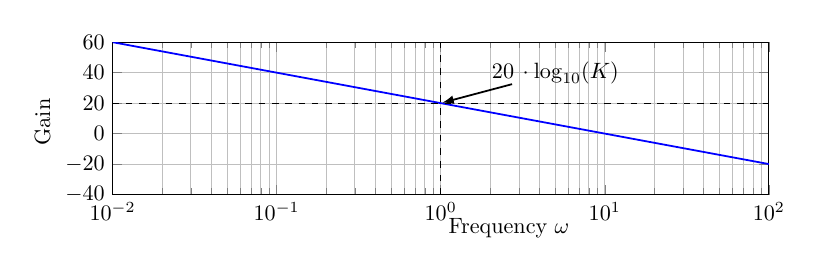
\begin{tikzpicture}
        [
            scale = 0.8,
            >=latex
        ]
        \begin{axis}
            [
                width=12cm,
                height=4cm,
                xmode=log,
                xmin=0.01, xmax=100, ymin=-40, ymax=60,
                x label style={anchor=west},
                xlabel=Frequency $\omega$,
                y label style={anchor=south},
                ylabel=Gain $\deci \bel$,
                xmajorgrids=true,
                xminorgrids=true,
                ymajorgrids=true
            ]

            % Plot
            \addplot[thick, color=blue, domain=0.01:100]{-20*log10(x)+20};
            
            % guide lines
            \addplot[dashed, color=black, domain=0.01:100]{20}; 
            \addplot [dashed, color=black] coordinates {(1, -40) (1, 60)};
           
            % Node / Label
            % \node (p) at (0.01, 20) {$20 \, \deci \bel \cdot \log_{10}(K)$};
            \node[inner sep=0pt] (p) at (1, 20) {};
            \node[inner sep=0pt] (q) at (5, 40) {$20 \, \deci \bel \cdot \log_{10}(K)$};

            \draw[->, thick, color=black] (q) -- (p);


        \end{axis}
        
    \end{tikzpicture}


    % Phase
    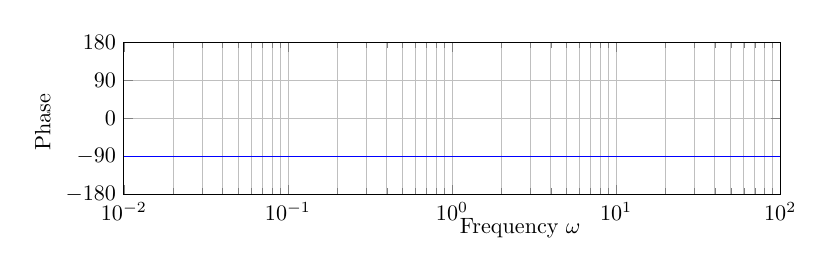
\begin{tikzpicture}
        [
            scale = 0.8,
            >=latex
        ]
        \begin{axis}
            [
                width=12cm,
                height=4cm,
                xmode=log,
                xmin=0.01, xmax=100, ymin=-180, ymax=180,
                x label style={anchor=west},
                xlabel=Frequency $\omega$,
                y label style={anchor=south},
                ylabel=Phase $\degree$,
                ytick={-180, -90, 0, 90, 180},
                % yticklabels={-180, -90, 0, 90, 180},
                xmajorgrids=true,
                xminorgrids=true,
                ymajorgrids=true
            ]
            
            % Phase
            \addplot[thick, color=blue, domain=0.01:100]{-90};
                
        \end{axis}
            
    \end{tikzpicture}
\end{center} 


\subsection{Bodediagramm eines Differenzierer}

Ein Differenzierer mit $G(s) = K \cdot s$ hat eine Nullstelle bei der Frequenz $\omega = 0$. Im Bodediagramm wird der Differenzierer so
dargestellt, dass bei Frequenz $\omega = 1$ die Verstärkung $20 \, \deci \bel \cdot \log_{10}(K)$ erreicht ist.
Die Steigung beträgt $20 \, \deci \bel / \mathrm{Dek}$ und die Phase ist konstant bei $\varphi = \frac{\pi}{2}$

\begin{center}
    % Gain
    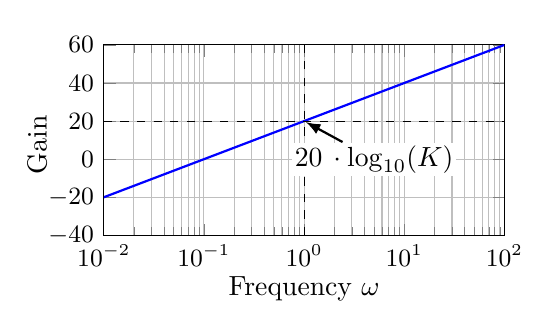
\begin{tikzpicture}
        [%
            scale = 1,
            >=latex
        ]
        \begin{axis}
            [%
                width=.55\columnwidth,
                height=4cm,
                % tick label style
                tick label style={font=\small},
                % x-axis
                xmode=log,
                xmin=0.01, xmax=100, ymin=-40, ymax=60,
                x label style={anchor=north, inner sep=0pt},
                xlabel=Frequency $\omega$,
                xmajorgrids=true,
                xminorgrids=true,
                % y-axis
                y label style={yshift=-1mm, anchor=south, inner sep=0pt},
                ylabel=Gain $\deci \bel$,
                ymajorgrids=true,
                yminorgrids=false
            ]
            % Plot
            \addplot[thick, color=blue, domain=0.01:100]{+20*log10(x)+20};
            
            % guide lines
            \addplot[dashed, color=black, domain=0.01:100]{20}; 
            \addplot [dashed, color=black] coordinates {(1, -40) (1, 60)};
           
            % Node / Label
            \node[inner sep=0pt] (p) at (1, 20) {};
            \node[fill=white, inner sep=1pt] (q) at (5, 0) {$20 \, \deci \bel \cdot \log_{10}(K)$};

            \draw[->, thick, color=black] (q) -- (p);
        \end{axis}
    \end{tikzpicture}
    % Phase
    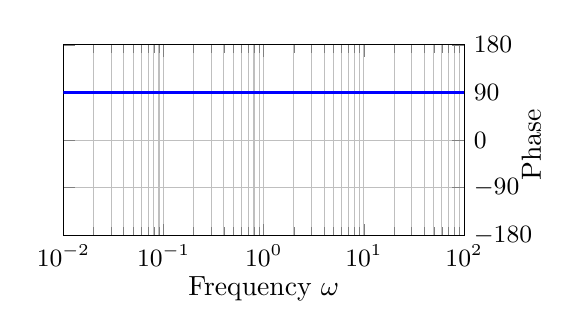
\begin{tikzpicture}
        [%
            scale = 1,
            >=latex
        ]
        \begin{axis}
            [%
                width=.55\columnwidth,
                height=4cm,
                % tick label style
                tick label style={font=\small},
                % x-axis
                xmode=log,
                xmin=0.01, xmax=100, ymin=-180, ymax=180,
                x label style={anchor=north, inner sep=0pt},
                xlabel=Frequency $\omega$,
                xmajorgrids=true,
                xminorgrids=true,
                % y-axis
                y label style={anchor=south, inner sep=0pt},
                ylabel=Phase $\degree$,
                yticklabel pos=right,
                ytick={-180, -90, 0, 90, 180},
                ymajorgrids=true,
                yminorgrids=false
            ]
            
            % Phase
            \addplot[thick, color=blue, domain=0.01:100]{90};
        \end{axis}
    \end{tikzpicture}
\end{center}

 


\subsection{z-Transformation}
\label{z-Transformation}

Die z-Transformation wird verwendet, um \textbf{diskrete} Signale in den Frequenzbereich zu transformieren.

\renewcommand{\arraystretch}{1.4}

\begin{center}
    \begin{tabular}{c | c}
        \textbf{Zeitbereich}    & \textbf{Frequenzbereich}  \\
        \midrule
        $u(k)$                  & $U(z)$                    \\
        $u(k-1)$                & $z^{-1} \cdot U(z) = \frac{1}{z} \cdot U(z)$ \\
        $u(k+1)$                & $z \cdot U(z)$
    \end{tabular}
\end{center}


\subsubsection{Z-Transformation mit Matlab}

\lstinputlisting{snippets/z_transformation.m}


\subsection{Fourier- bzw. Laplace-Transformation}

Die Fourier- und die Laplace-Transformation werden verwendet, um \textbf{kontinuierliche} Signale ein den Frequenzbereich zu transformieren.

\begin{center}
    \begin{tabular}{c |c | c}
        \textbf{Zeitbereich}            & \textbf{Frequenzbereich (Fourier)}                & \textbf{Frequenzbereich (Laplace)}    \\
        \midrule
        $u(t)$                          & $U(\jimg \omega)$                                 & $U(s)$                                \\
        $\int u(\tau) \, \diff \tau$    & $\frac{1}{\jimg \omega} \cdot U(\jimg \omega)$    & $\frac{1}{s} \cdot U(s)$              \\
        $\frac{\diff}{\diff u(t)}$      & $\jimg \omega \cdot U(\jimg \omega)$              & $s \cdot U(s)$
    \end{tabular}
\end{center}
\renewcommand{\arraystretch}{1}
    \end{layout}
\end{document}